\documentclass[class=book, crop=false, oneside]{standalone}
\usepackage[subpreambles=true]{standalone}

\usepackage{../../style}
\usepackage{../../set-citations}

\graphicspath{{./assets/images/}}

% arara: pdflatex: { synctex: yes, shell: yes }
% arara: latexmk: { clean: partial }
%! arara: clean: { extensions: [sta] }
\begin{document}

\chapter{Aritmetica dei calcolatori}

\section{Informazione nei computer}

\subsection{I transistor}

\begin{wrapfigure}{r}{0.4\textwidth}
	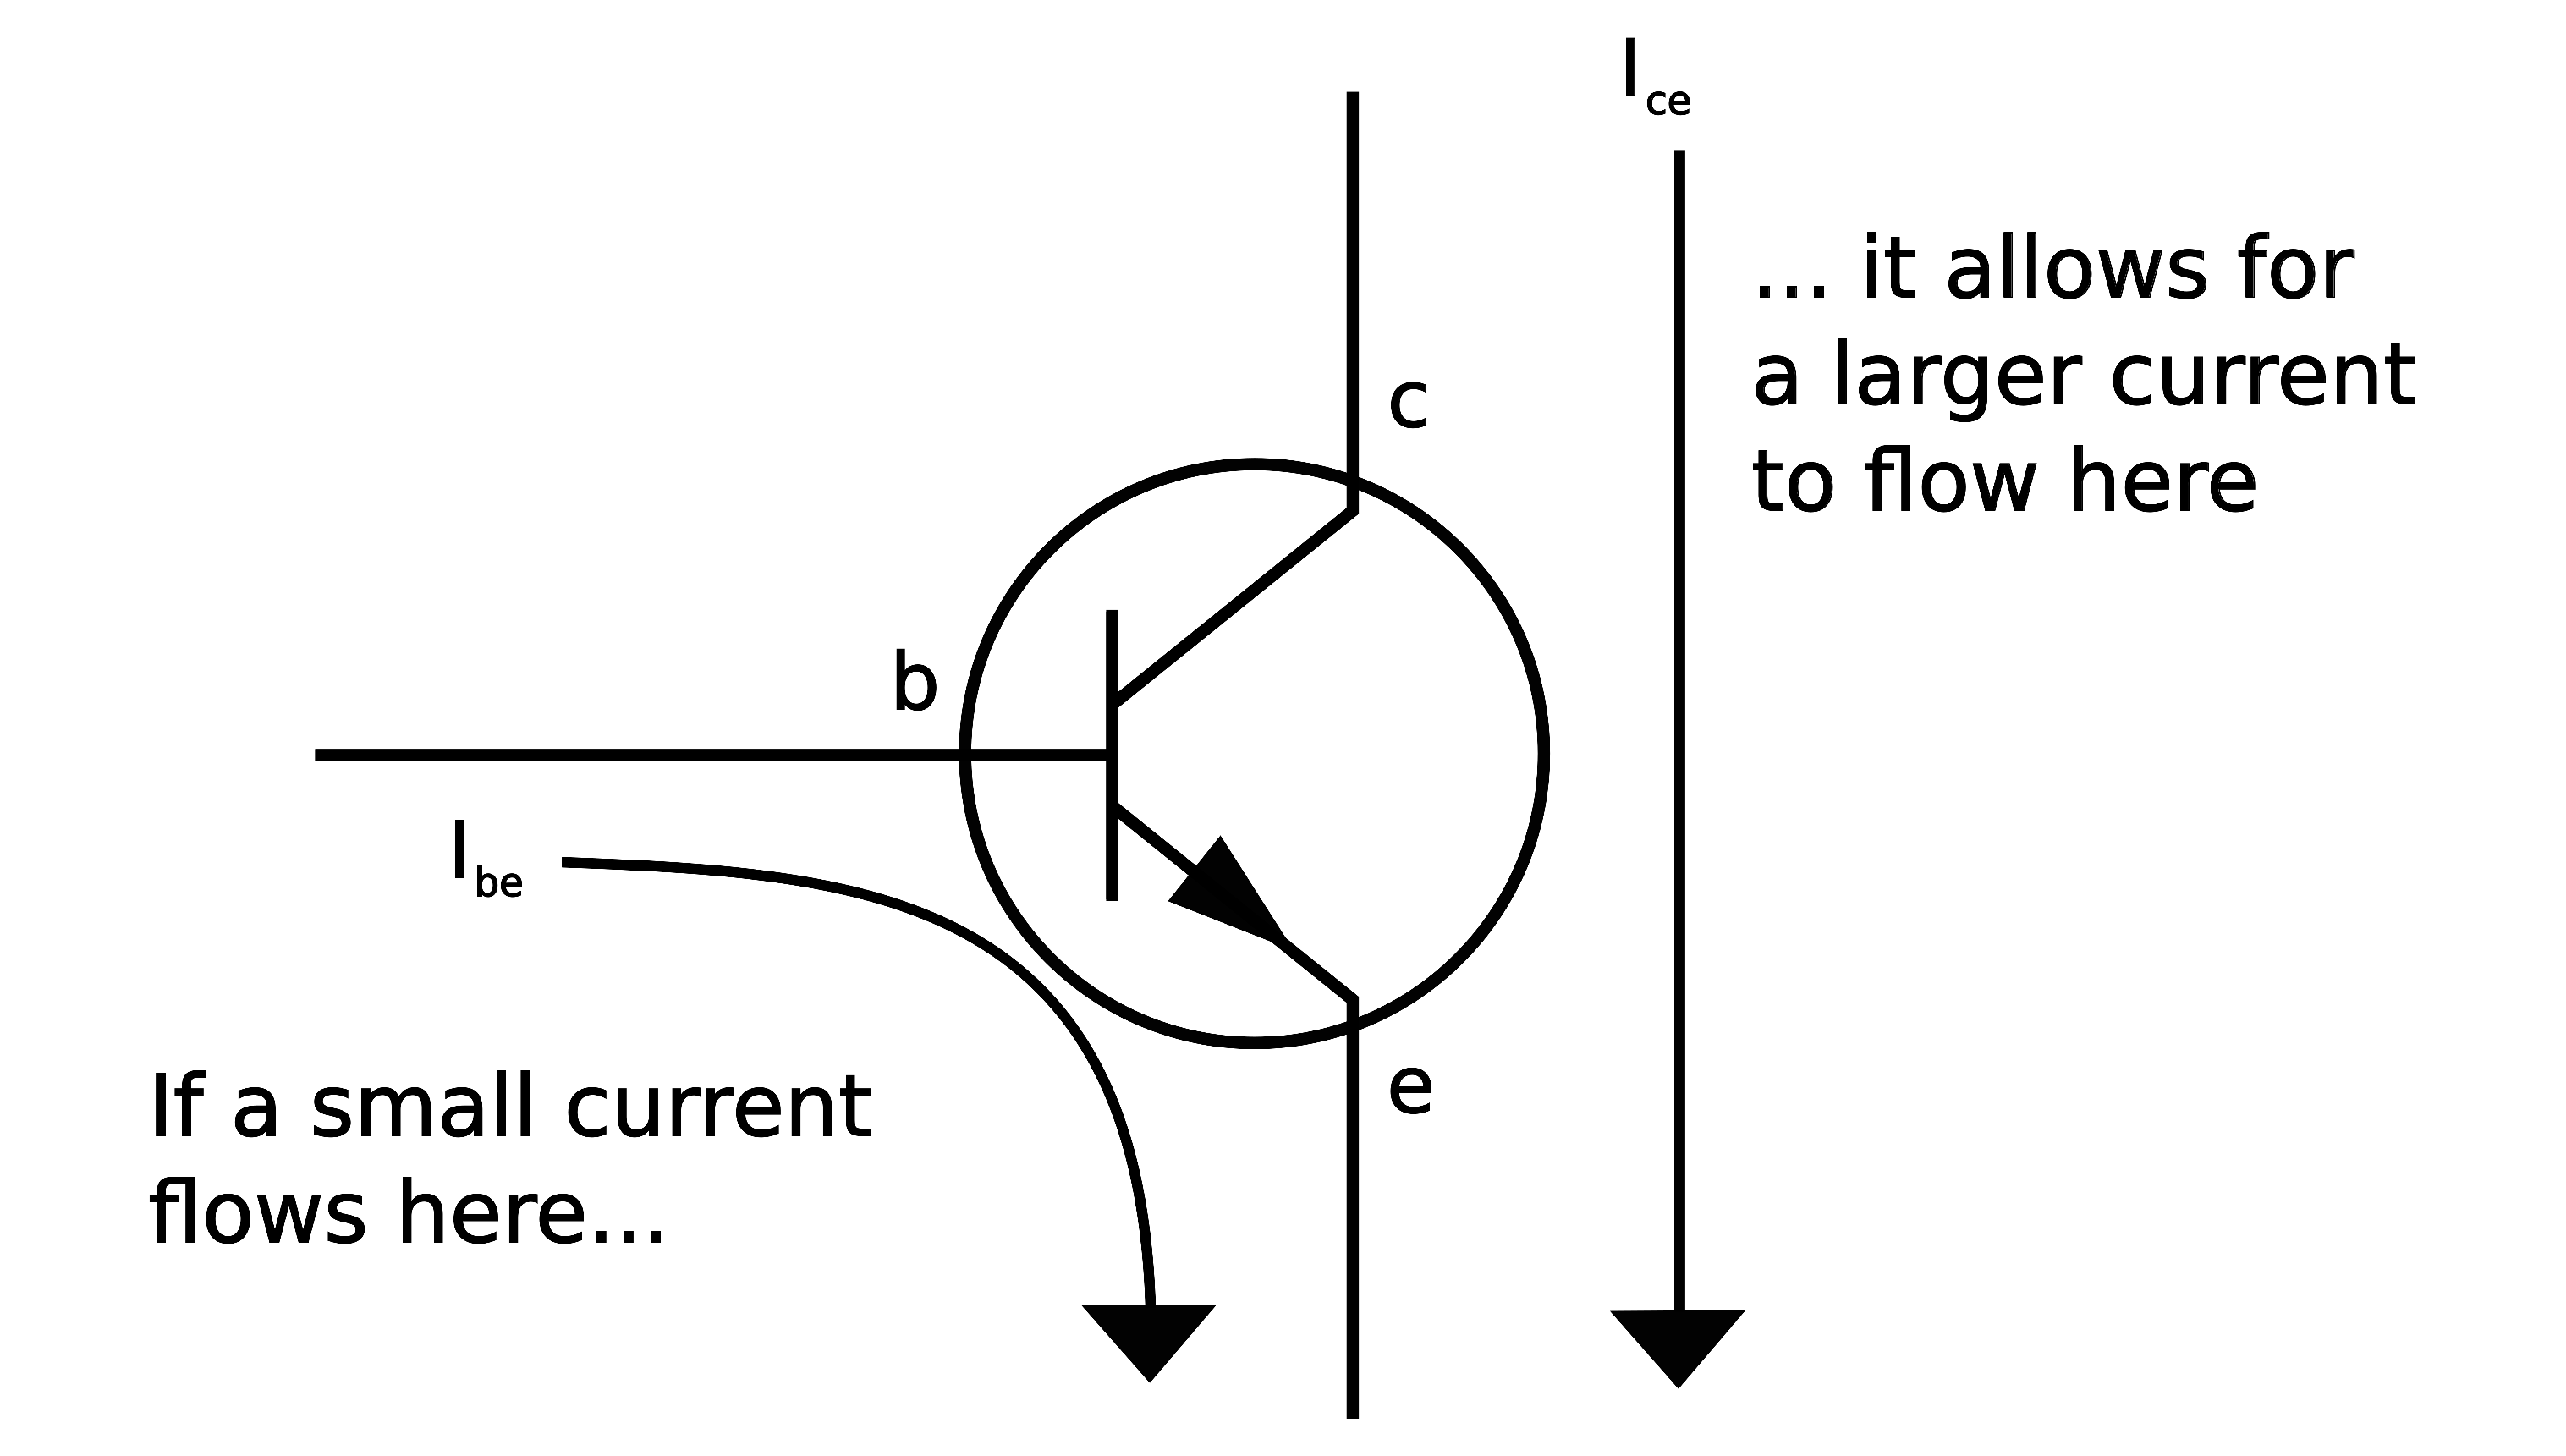
\includegraphics[width=\linewidth]{transistor.eps}
	\label{fig:transistor}
	\centering
\end{wrapfigure}

Tutti i computer moderni sono composti da \emph{transistor} (detti anche triodi), delle strutture bistabili: possono assumere due stati come un interruttore, 0 (spento) e 1 (acceso). Molti \emph{transistor} collegati tra loro in una sorta di matrice possono rappresentare delle serie di porte logiche, ed è questa la struttura che sta alla base dell'architettura dei moderni calcolatori.

Un computer memorizza (e manipola) solo sequenze di 0 e 1 (sequenze di bit); anche l’ENIAC funzionava allo stesso modo, solo che al posto dei \emph{transistor} era composto da \emph{valvole termoioniche}, che non erano differenti nel funzionamento (assumono sempre i due stati descritti in precedenza, solo più lentamente).

\subsection{Interpretazione delle informazioni} In seguito le sequenze di bit che i computer elaborano/memorizzano possono essere interpretate in tantissimi modi diversi, tra cui numeri, caratteri, suoni, immagini, istruzioni e molti altri. Alla base di tutte le interpretazioni che si possono dare alle stringhe di simboli (che nel caso del computer sono proprio i due stati del bit) sta il concetto di codifica. La \emph{codifica} è appunto uno schema, una legge, un \emph{mapping} che permette prima di tradurre, poi di interpretare stringhe di simboli.

Nell’ambito dell’IT le codifiche sono fortemente caratterizzate dalla lunghezza (dal numero di bit) delle “parole” elementari della codifica. Ad esempio, per rappresentare tutti i caratteri (tabella ASCII estesa) utilizziamo  8 bit (256 caratteri). Si osservi che essendo i \emph{transistor} sistemi bistabili la base 2 (con cifre 0 e 1) è perfetta per rappresentare la codifica dei dati memorizzati/elaborati da essi.

\section{I numeri}
Limitiamoci al caso dei numeri per spiegare il concetto di \emph{codifica}. Ricordiamo che i metodi di rappresentazione numerica che studiamo sono posizionali, ovvero il peso di ogni cifra varia in base alla posizione che essa occupa. In generale se una base è composta da \(B\) elementi essa ha \(B\) cifre (da 0 a \(B\)) utilizzate per scrivere ogni numero. Questa formula ci restituisce il valore di ogni numero scritto in una qualsiasi base \(B\):
\begin{equation*}
	c_{i} c_{i-1} c_{i-2}... c_{0}=c_{i}\cdot B^{i}+...+c_{0}\cdot B^{0}
\end{equation*}
dove \(c_{i}\) è la cifra in posizione \(i\).

\subsection{Regole di conversione tra basi}
Vediamo ora come operare la conversione tra le principali basi:
\begin{itemize}
	\item \emph{da base 2 a base 16}: partendo da destra, si dividano le cifre binarie in gruppi da 4 cifre ciascuno, e ognuno di questi corrisponderà a una cifra esadecimale; qualora il numero di cifre binarie non sia divisibile per 4, si completi con degli 0 in modo da ottenere gruppi da 4 (\emph{esempio}: \((11011)_{2}\) diventerà \((0001\text{ }1011)_{2}\), ovvero \((1B)_{16}\));
	\item \emph{da base 2 a base 8}: analogamente, si dividano le cifre binarie in gruppi da 3 cifre ciascuno, e ognuno di questi corrisponderà a una cifra ottale;
	\item \emph{da una qualsiasi base B a base 10}: come visto sopra, si moltiplichi ogni cifra $c_{i}$ per $B^{i}$, dipendentemente dalla sua posizione;
	\item \emph{da base 10 a una qualsiasi base B}:
	\begin{enumerate}[noitemsep,nolistsep]
		\item si consideri un numero \(x_{10}\) e una base \(B\);
		\item si divida \(x\) per \(B\);
		\item il resto della divisione è la cifra da inserire a sinistra nel numero convertito;
		\item si assegni a \(x\) il quoziente della divisione;
		\item si torni al punto 2 e si ripeta finché \(x\neq0\).
	\end{enumerate}
\end{itemize}
\begin{figure}[h!]
	\centering
	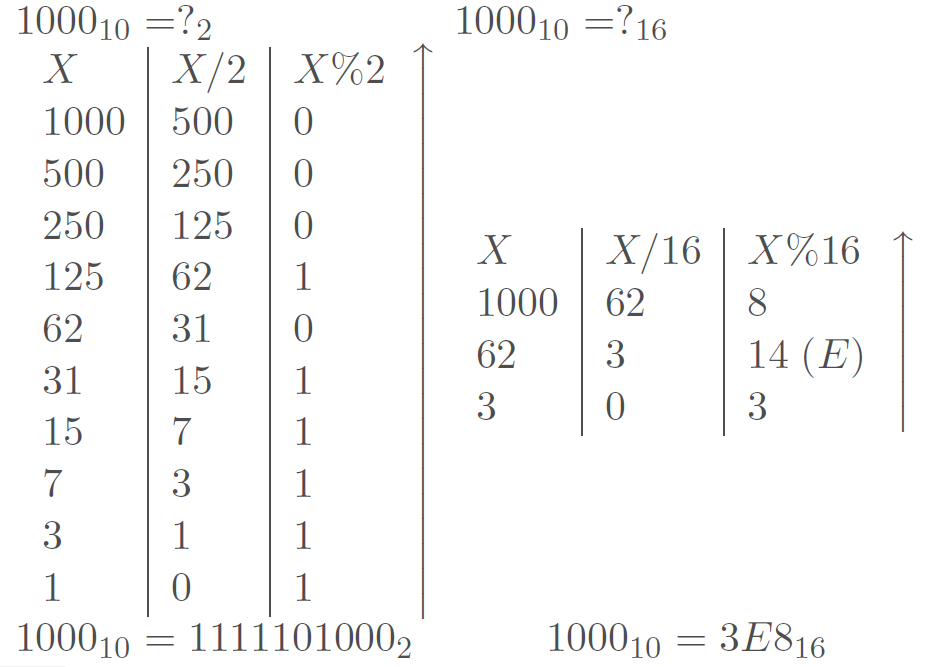
\includegraphics[width=0.5\textwidth,keepaspectratio]{esempi_conversioni.png}
	\caption{Alcuni esempi di conversione}
\end{figure}

\subsection{I naturali}
Nella codifica binaria un numero naturale è rappresentato su \emph{k} cifre binarie, dove con \emph{k} cifre si possono rappresentare i numeri tra 0 e \(2^{k}-1\). La codifica più comune per gli interi spesso usa i byte, sequenze di 8 bit, che tuttavia richiedono molte cifre per rappresentare un numero e quindi spesso, per semplificare la lettura, si usa scrivere i numeri in esadecimale (quindi scrivendo un quarto delle cifre rispetto alla binaria).

\paragraph*{Somma e sottrazione}
Le operazioni somma e sottrazione funzionano allo stesso modo del sistema utilizzato nella numerazione decimale con il riporto. Si guardino gli esempi qui sotto riportati, già di per sè esplicativi del processo:
\vspace{10px}

\begin{table}[h!]
	\centering
	\subimport{assets/tables/}{es_somma.tex}
	\caption{Esempio di somma}
\end{table}
\begin{table}[h!]
	\centering
	\subimport{assets/tables/}{es_diff.tex}
	\caption{Esempio di differenza}
\end{table}

\paragraph*{Moltiplicazione}
La moltiplicazione in base binaria si può semplificare con il metodo dello shifting, che è più facile illustrare con un esempio:
\begin{table}[H]
	\centering
	\subimport{assets/tables/}{es_prod.tex}
	\caption{Esempio di prodotto}
\end{table}
Si noti che quando è presente un 1 si riscrive il numero (nella posizione corrispondente) mentre  quando è presente uno 0 semplicemente non si scrive nulla (e si va solo avanti con le posizioni).

\subsection{Gli interi}
Finora abbiamo visto come si codificano solo i numeri naturali, ma esistono metodi di codifica che permettono di rappresentare anche i numeri negativi (quindi l’insieme degli interi). Le tecniche più comuni sono: modulo e segno, complemento a 1 (\emph{CA1}) e complemento a 2 (\emph{CA2}).

\paragraph*{Codifica con Modulo e Segno}
Si usano \(k-1\) bit per rappresentare il valore assoluto (modulo) del numero  ed un bit per codificare il segno (0 per i positivi, 1 per i negativi). In questo modo con k bit si possono codificare valori tra \(-2^{k-1}+1\) e \(+2^{k-1}-1\).\\
\emph{NB}: esistono due codifiche per lo \(0\), \(-0\) e \(+0\), e questo è un spreco.

\paragraph*{Codifica in Complemento a 1}
Il primo bit indica sempre il segno e per ottenere l'opposto di un numero positivo si invertono tutti gli 0 in 1 e gli 1 in 0 (e lo stesso si fa per ottenere l’opposto di un numero negativo). Si hanno ancora due rappresentazioni per \(+0\) e \(-0\) (rispettivamente, utilizzando 4 bit, \(0000\) e \(1111\)). È più facile da sommare rispetto al modulo e segno ma solo se il bit significativo non dà riporto.\\
Quando si sommano due numeri in \emph{CA1}:
\begin{itemize}[noitemsep]
	\item si deve verificare che i riporti delle prime due cifre significative siano uguali, altrimenti il numero che si ottiene non è rappresentabile in CA1 su k bit.
	\item alla fine si deve sommare il riporto della prima cifra al risultato ottenuto (ultima riga).
\end{itemize}

\begin{figure}[h!]
	\centering
	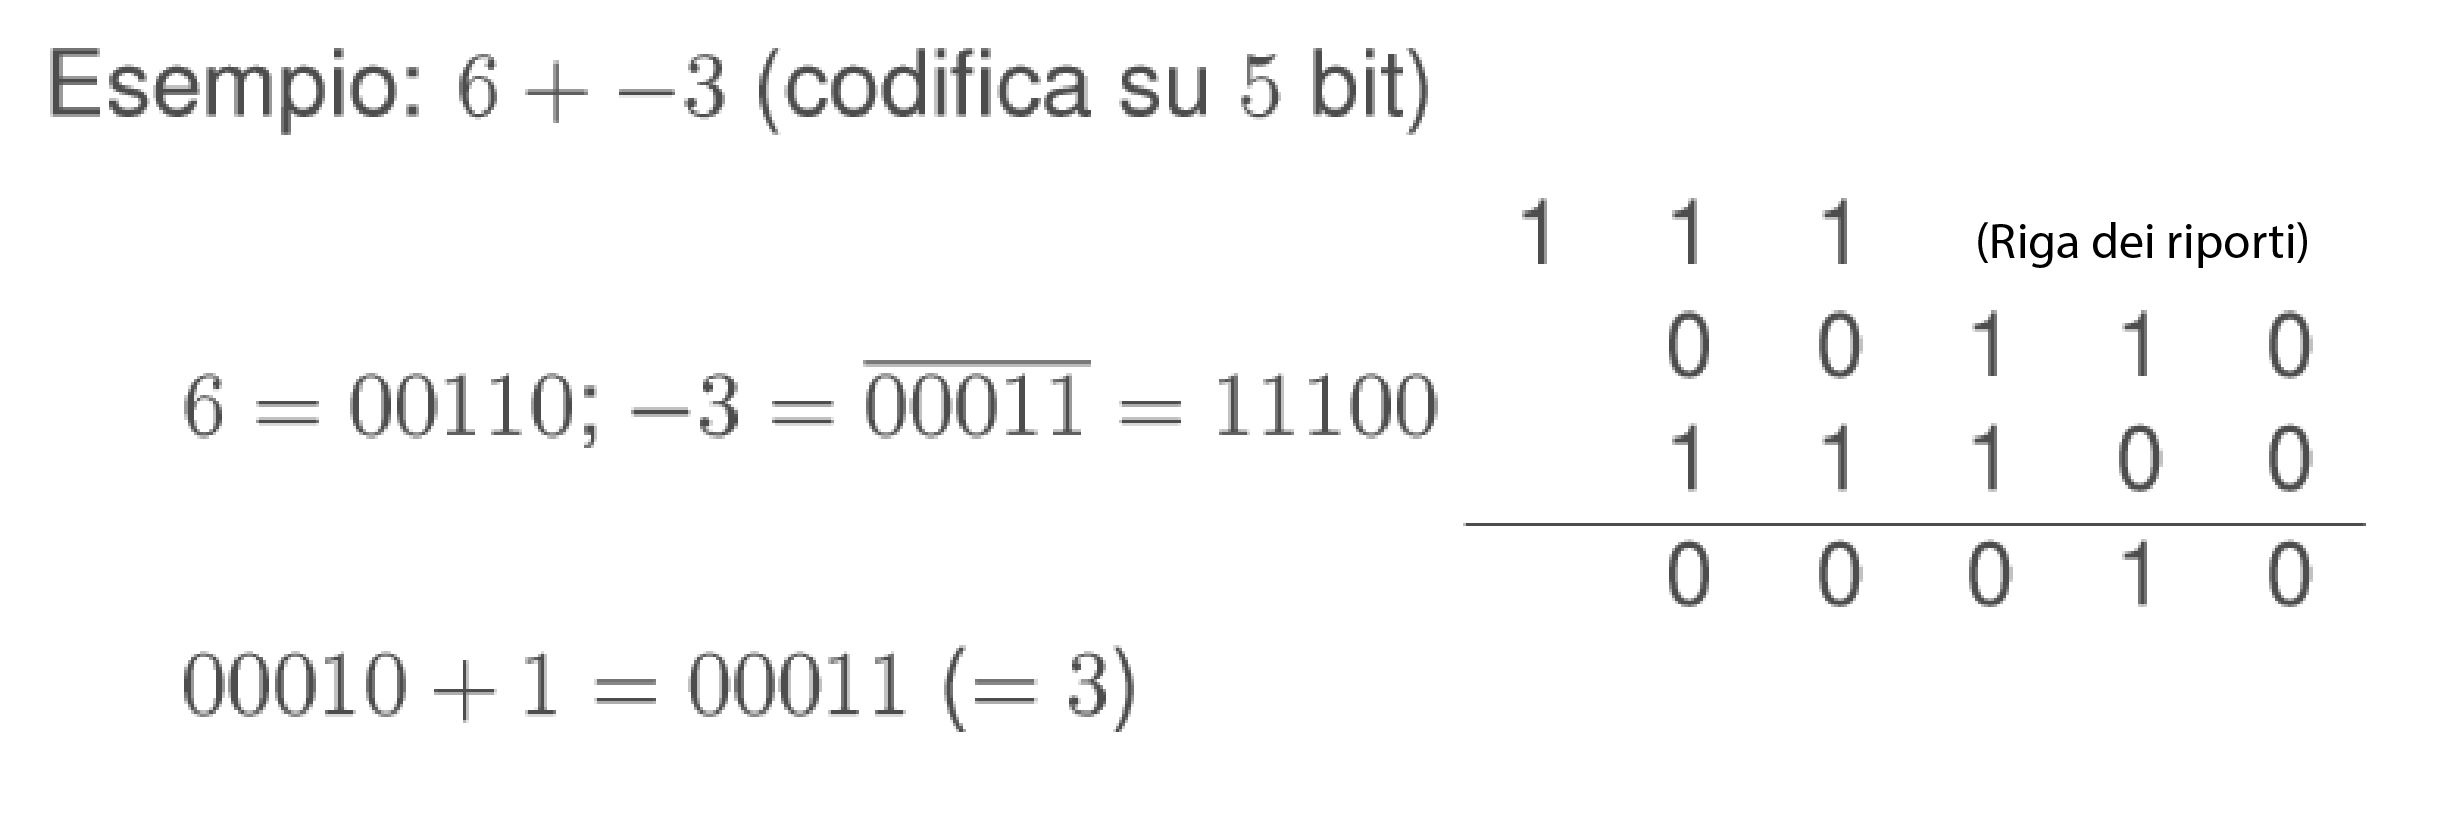
\includegraphics[width=0.7\textwidth,keepaspectratio]{Somma-CA1.png}
	\caption{Esempio di somma in CA1}
\end{figure}

\paragraph*{Codifica in Complemento a 2}
Per tradurre un numero da intero con segno a complemento a 2 (\emph{CA2}) basta invertire tutti i bit e poi sommare 1. Viceversa, per convertire da \emph{CA2} a binario, si sottrae 1 e poi si invertono tutti i bit. Ancora una volta il bit più significativo indica il segno, ma in questo caso la codifica dello 0 è unica, quindi con \(k\) bit si possono rappresentare i numeri da \(-2^{k-1}\) a \(2^{k-1}-1\).

\subsubsection{Somma algebrica in Complemento a 2}
L'utilizzo della codifica \emph{CA2} permette di eseguire somme algebriche senza alcuna differenza operativa, ma rende necessario prestare attenzione all'\emph{overflow}. Con il termine \emph{overflow} si intende la situazione in cui, date in input delle informazioni codificate in un numero \(k\) di bit arbitrariamente scelto, lo stesso numero \(k\) di bit non è sufficiente a codificare le informazioni in output.

Diamo subito un esempio: supponiamo di voler eseguire \(-64-8\) utilizzando il \emph{CA2} e \(k=7\) bit. Ricordiamo che:
\begin{align*}
-64=1000000_{2}=\overline{1000000}+1=0111111+1=1000000 \text{ in \emph{CA2}}\\
-8=0001000_{2}=\overline{0001000}+1=1110111+1=1111000 \text{ in \emph{CA2}}
\end{align*}
A questo punto eseguiamo la somma algebrica:
\begin{table}[H]
	\centering
	\subimport{assets/tables/}{overflow_CA2.tex}
\end{table}
Si noti che il numero fra parentesi indica l'ultimo riporto, che chiaramente non possiamo inserire poiché sforerebbe i 7 bit.\\
Osserviamo così che, per \(k=7\) bit, \(-64-8=0111000_{2}=56_{10}\), che ovviamente non ci piace; concludiamo quindi che la somma algebrica \(-64-8=-72\) \emph{non} è rappresentabile con soli \(k=7\) bit.

In generale possiamo dire che, dati due numeri \(a\) e \(b\) aventi lo stesso segno, avremo problemi di \emph{overflow} se:
\begin{itemize}
	\item \(a+b>2^{k-1}-1\);
	\item \(a+b<-2^{k-1}\).
\end{itemize}
ricordando che \(-2^{k-1}\le a,b\le 2^{k-1}-1\).

\subsection{Aritmetica modulare}
Inconsapevolmente utilizziamo l'\emph{aritmetica modulare} quasi continuamente, nella nostra quotidianità; l'esempio più comune è quando sommiamo le ore, che sono organizzate in modulo 24 (da cui la denominazione ufficiosa di "Matematica dell'orologio"), ma anche minuti e secondi (modulo 60) e gli angoli (modulo 360).

Diamone una descrizione intuitiva: fissato un numero \(n\) finito di valori, arrivato al numero più grande (\(n-1\)), al successivo avrò che \((n-1)+1=0\). Per completezza, forniamo ora la relazione di equivalenza di due numeri in modulo \(n\):
\begin{equation*}
	a\equiv b \Longleftrightarrow a\%n=b\%n
\end{equation*}

Quando eseguiamo delle operazioni sui numeri in base 2 su \(k\) bit, stiamo lavorando in un ambiente in modulo \(2^{k}\), e calcolando \(a+b\) stiamo in realtà trovando \((a+b)\%2^{k}\), e i due valori saranno uguali se e solo se \(a+b<2^{k}\), perché altrimenti ogni valore successivo ricomincerebbe da 0: questo è l'\emph{overflow}. In particolare, quando lavoriamo su numeri interi in \emph{CA2}, dobbiamo ricordare che, se \(-2^{k-1}\le a+b\le 2^{k-1}-1\) non avremo \emph{overflow}, altrimenti:
\begin{itemize}
	\item se \(a+b>2^{k-1}-1\), otterremo \(a+b+2^{k}\) \(\longrightarrow\) \emph{overflow};
	\item se \(a+b<-2^{k-1}\), otterremo \(a+b-2^{k}\) \(\longrightarrow\) \emph{overflow}.
\end{itemize}

\subsection{I reali}
Non è sempre semplice codificare un numero reale \(\alpha \in \mathbb{R}\), poiché di questo insieme fanno parte i numeri cosiddetti \emph{irrazionali}, che presentano infinite cifre non periodiche dopo la virgola (si pensi ad esempio a \(\pi=3,14159...\), o \(e=2.71828...\), o ancora \(\sqrt{2}=1.41421...\)). Alcuni numeri non possono quindi essere rappresentati con un numero finito di bit, per cui ne rappresenteremo solo un'approssimazione, e per farlo abbiamo sviluppato due metodi: la rappresentazione a \emph{virgola fissa} (\emph{fixed point}) e quella a \emph{virgola mobile} (\emph{floating point}).

\subsubsection{Codifica in virgola fissa} Questo sistema di codifica prevede che, posto un numero \(k\) di bit per la rappresentazione del numero, si impieghino \(k-f\) bit per rappresentarne la parte intera, e i restanti \(f\) bit per rappresentarne la parte razionale:
\begin{equation*}
	\overbrace{\underbrace{c_{k-1}c_{k-2}\cdots c_{f}}_\text{$k-f$}\underbrace{\cdot c_{f-1}\cdots c_{0}}_\text{$f$}}^\text{$k$}
\end{equation*}
Possiamo scrivere una formula generale più compatta. Supponiamo di voler convertire un numero $x_{10}$:
\begin{equation*}
 	x_{10}=\sum_{i=0}^{k-1} c_{i}B^{i-f}=\sum_{i=0}^{k-1} c_{i}B^{i}\cdot B^{-f}=(\sum_{i=0}^{k-1} c_{i}B^{i})\cdot B^{-f}
 \end{equation*}
Detta in altri termini, convertiamo il numero da base 10 come se non avesse la virgola e poi moltiplichiamo per \(B^{-f}\). Presentiamo vantaggi e svantaggi di questo tipo di codifica:
\begin{itemize}[noitemsep]
	\item le operazioni si possono svolgere senza alcuna differenza, se non l'accortezza di scalare il risultato;
	\item il peso per la CPU è ridotto;
	\item non ci sono errori di approssimazione, \emph{se il valore è rappresentabile};
	\item iniziamo ad avere problemi quando lavoriamo con un ampio spettro di ordini di grandezza.
\end{itemize}

\subsubsection{Codifica in virgola mobile}
Un qualsiasi numero reale può essere scritto anche nella forma \(x=M\cdot B^{exp}\) dove M si dice \emph{mantissa}, \emph{exp} \emph{esponente} (effettivo dei calcoli) e B è la base della rappresentazione (che nel nostro caso è la leggendaria base 2).

Questo metodo di rappresentazione, molto simile alla notazione scientifica standard, è implementato anche nell'informatica in più modi diversi ma alla base di tutti si riconosce lo stesso schema: \(x\) può essere rappresentato su \(k\) bit utilizzando \(m\) bit per il campo mantissa M ed \(e=k-m\) bit per il campo esponente E (esponente memorizzato, attenzione: è diverso dall'esponente effettivo dei calcoli); quest'ultimo permette in un certo senso di "spostare" la virgola; con esponenti "piccoli" si avranno \(x\) "piccoli" e viceversa con esponenti "grandi" si avranno \(x\) "grandi".\\
Lo standard più comunemente utilizzato è l'IEEE 754 che, nei numeri \emph{float} a precisione singola (dove si usano 32 bit), ha questa struttura:
\begin{table}[h!]
	\centering
	\begin{tabular}{|l|l|l|}
		\hline
		\multicolumn{1}{|c|}{1 bit} & \multicolumn{1}{c|}{8 bit} & \multicolumn{1}{c|}{23 bit} \\ \hline
		Bit di segno                & E (esponente memorizzato)    & Mantissa                    \\ \hline
	\end{tabular}
\end{table}


Il bit di segno ha la funzione che già conosciamo, mentre il campo \(E\) può contenere valori compresi tra 0 e 255 (se non si tratta di un \emph{float} a precisione singola i valori sono compresi tra 0 e \(2^{e-1}-1\))% ($-2^{e-1}+1 < E \le 2^{e-1}-1$)
; questi ultimi due valori vengono utilizzati per funzioni speciali, mentre i valori da 1 a 254 compresi codificano l'\emph{esponente effettivo dei calcoli}, che diremo \emph{exp}\footnote{La notazione \emph{exp} è stata introdotta da noi autori della dispensa perchè ci è sembrata più chiara ed agile di quella utilizzata nelle slides, chiediamo venia se questo genererà confusione.}, in questo modo:
\begin{equation*}
	exp=E-(2^{e-1}-1)
\end{equation*}
Il numero \(2^{e-1}-1\) viene detto \emph{bias} e nel nostro caso è \(127\), per cui \(\textrm{exp}=E-127\). L'ultimo campo, la \emph{mantissa}, codifica un numero intero.

\paragraph{Come calcolare il valore di un float} Il primo bit è utilizzato per indicare il segno, i successivi 8 per $E$ e i restanti 23 per la mantissa. La decodifica in decimale assume due forme in base al valore di \(E\):
\begin{itemize}
	\item se \(E=0\), allora il numero in base 10 è \(x_{10}=0.M \cdot 2^{(exp+1=-126)}\);
	\item se \(E>0\), allora il numero in base 10 è \(x_{10}=1.M \cdot 2^{exp}\), dove \emph{exp} è definito come qui sopra descritto.
\end{itemize}
Nel primo di questi due casi i numeri si dicono \emph{denormalizzati}, essi rappresentano tutti i numeri compresi tra \(1.4\cdot10^{-45}\) e \(1.1754942\cdot10^{-38}\); nel secondo caso i numeri si dicono \emph{normalizzati} [questa distinzione è stata aggiunta per migliorare la precisione della notazione con numeri molto vicini allo 0].

Per tradurre in decimale un numero in virgola mobile si deve quindi per prima cosa determinare il segno, poi si calcola l'esponente effettivo dei calcoli (\(exp=E-\text{\emph{bias}}\)) e da qui, simmetricamente a prima, si procede in due modi:
\begin{itemize}
	\item se \(exp\neq-\text{\emph{bias}}\) si parla di numero \emph{normalizzato} e quindi si aggiunge un bit 1 alla mantissa in modo da ottenere il numero \(1.M\) e si sposta la virgola di \emph{exp} posizioni e per completare il tutto si traduce il numero binario (in virgola fissa) così ottenuto in decimale;
	\item se \(exp=-\text{\emph{bias}}\) si parla di numero \emph{denormalizzato} e quindi si aggiunge un bit 0 alla mantissa in modo da ottenere $0.M$ e come prima si sposta la virgola di (\(\text{\emph{exp}+1}\)) posizioni e poi si decifra il numero (binario in virgola fissa) così ottenuto;
\end{itemize}
Ripetiamo ancora una volta il procedimento per chiarezza: stabilito quale delle precedenti due opzioni riguarda il nostro caso spostiamo la virgola di \emph{exp} posizioni nel numero \(1.M\) oppure \(0.M\) (verso destra se \(exp>0\) e viceversa), ed in conclusione decodifichiamo il numero ottenuto come se fosse un binario in virgola fissa.

\subsubsection{Tabella riassuntiva}
Ecco una breve tabella riassuntiva dell'interpretazione delle stringhe nella rappresentazione IEEE 754:
\begin{table}[h!]
	\centering
	\subimport{assets/tables/}{floating_point.tex}
	\caption{Riepilogo floating point}
\end{table}

\subsubsection{Esempio di decodifica di un numero in virgola mobile}
Si traduca in IEEE 754 il numero \((01000010 10011011 10000000 00000000)_2\). Spacchettiamolo nei vari campi:
\begin{table}[h!]
	\centering
	\begin{tabular}{|l|l|l|}
		\hline
		\multicolumn{1}{|c|}{MSB} & \multicolumn{1}{c|}{Esponente} & \multicolumn{1}{c|}{Mantissa} \\ \hline
		0 & 10000101 & 00110111000000000000000\\\hline
	\end{tabular}
\end{table}
Procediamo ora alla traduzione.
\begin{enumerate}
	\item Osserviamo che il numero è positivo, poiché il bit di segno è 0.
	\item L'esponente effettivo dei calcoli \emph{exp} è
	\begin{equation*}
		E - 127 = E - \text{bias} = 10000101 - 01111111 = 133 - 127 = 6
	\end{equation*}
	L'esponente è diverso da zero, perciò si tratta di un numero normalizzato.
	\item La mantissa va moltiplicata per \(2^{exp} = 2^{6}\) e, poiché il numero è normalizzato, devo considerare $1.M$:
	\begin{equation*}
		1.M \cdot 2^{6} = 1.00110111000000000000000 \cdot 2^{6} = 1001101.11
	\end{equation*}
	\item A questo punto convertiamo il risultato ottenuto come fosse in virgola fissa:
	\begin{equation*}
		2^{6} + 2^{3} + 2^{2} + 2^{0} + 2^{-1} + 2^{-2} = 77.75
	\end{equation*}
\end{enumerate}

\end{document}
